\section{Visualization}
In this part, we visualize the forecasting results of \method compared with the state-of-the-art and representative methods (e.g., GPT4TS~\citep{zhou2023one}, PatchTST~\citep{nie2022time}, and Autoformer~\citep{wu2021autoformer}) in various scenarios to demonstrate the superior performance of \method. 

In \shortautoref{fig:visual_etth1} and \shortautoref{fig:visual_m4}, the long-term (input-96-predict-96) and short-term (input-36-predict-36) forecasts of various approaches are compared with the ground truth. Here, \method showcases forecasting accuracy that is notably superior compared to GPT4TS, PatchTST, and a classical Transformer-based method, Autoformer. 

We also offer visual comparisons of the forecasting results in both few-shot and zero-shot scenarios, as depicted in \shortautoref{fig:visual_ettm1} and \shortautoref{fig:visual_etth1_etth2}. We adhere to the long-term (input-96-predict-96) forecasting setup in both cases. \method exhibits remarkable superiority in forecasting with limited data—a fact that becomes particularly salient when compared to GPT4TS.

\clearpage
\newpage

\begin{figure*}[!htbp]
\begin{center}
\centerline{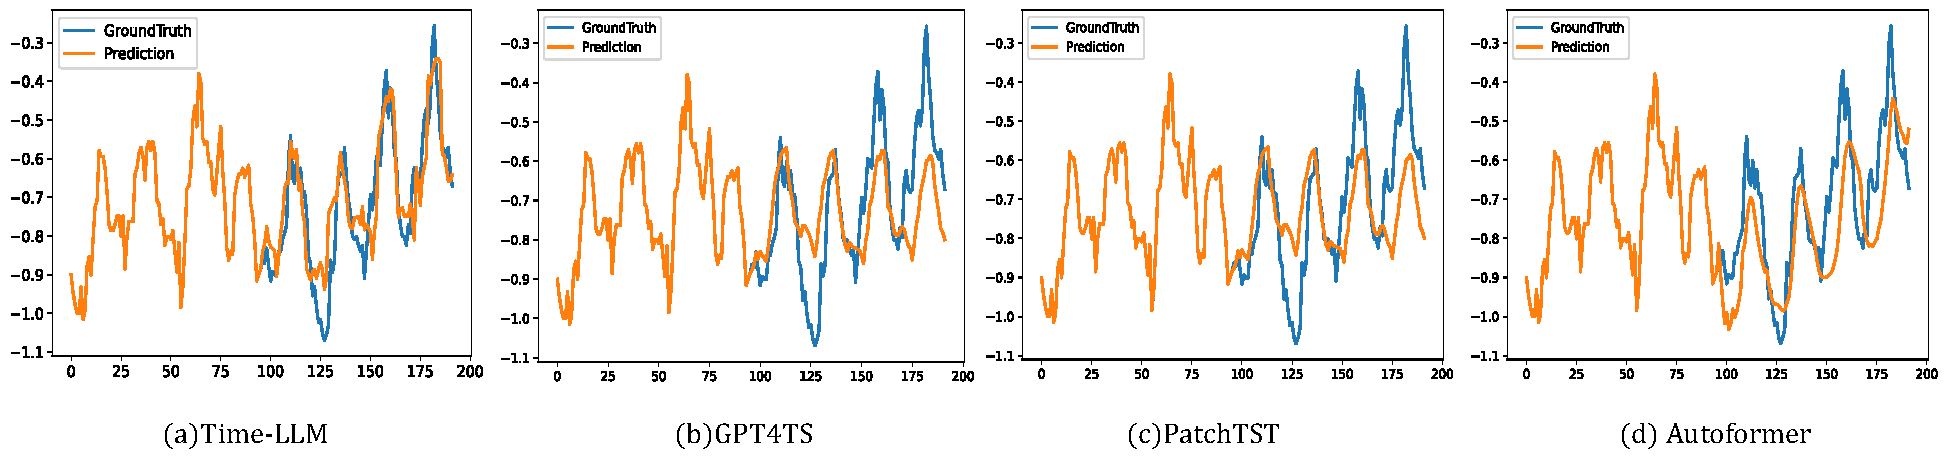
\includegraphics[width=\columnwidth]{figures/visual_long.pdf}}
	\caption{Long-term forecasting cases from ETTh1 by different models under the input-96-predict-96 settings. \textcolor{blue}{Blue} lines are the ground truths and \textcolor{orange}{orange} lines are the model predictions.}
	\label{fig:visual_etth1}
\end{center}
\vspace{-20pt}
\end{figure*}

\begin{figure*}[!htbp]
\begin{center}
\centerline{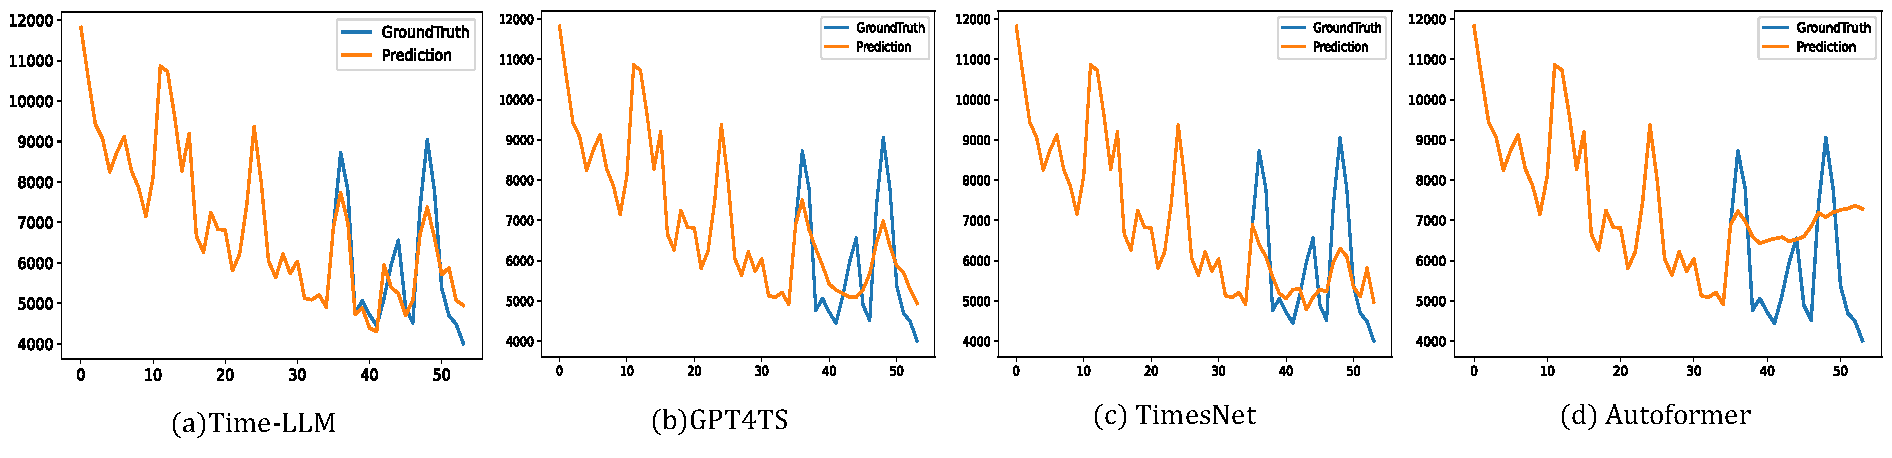
\includegraphics[width=\columnwidth]{figures/visual_m4.pdf}}
	\caption{Short-term forecasting from the M4 dataset by different models under the input-36-predict-18 settings.}
	\label{fig:visual_m4}
\end{center}
\vspace{-20pt}
\end{figure*}

\begin{figure*}[!htbp]
\begin{center}
\centerline{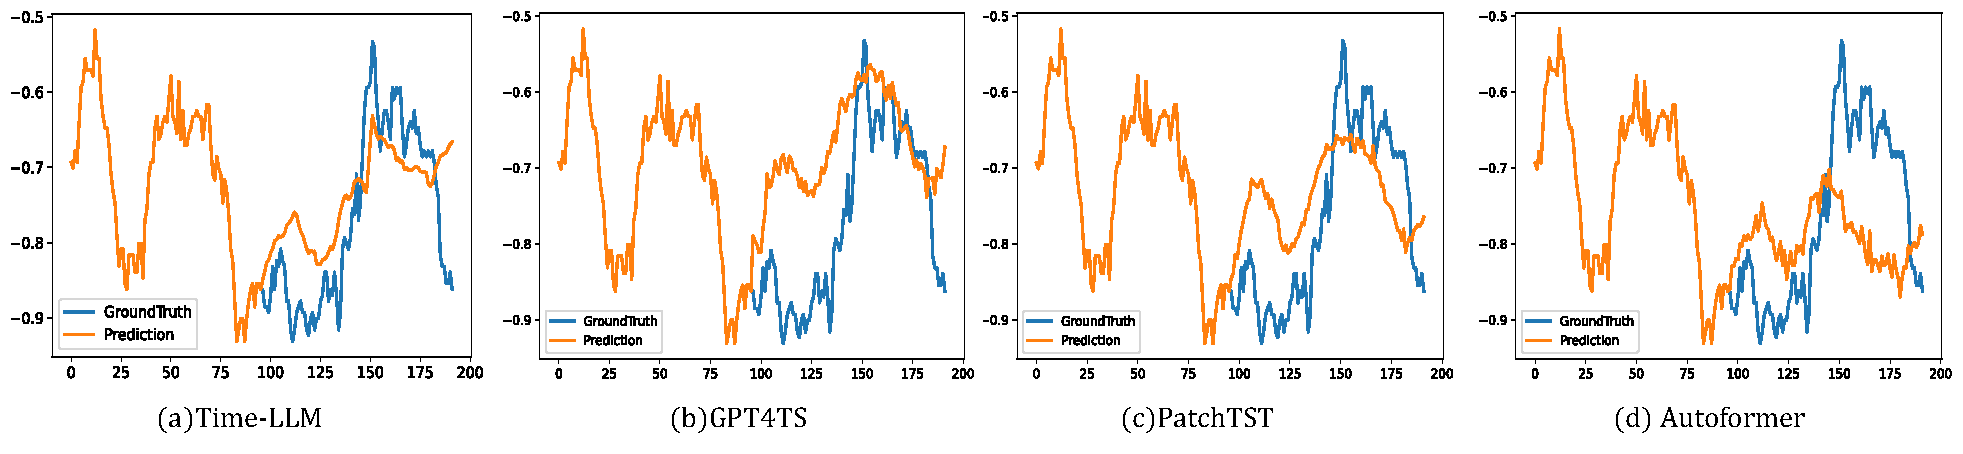
\includegraphics[width=\columnwidth]{figures/visual_few.pdf}}
	\caption{Few-shot forecasting cases from ETTm1 by different models under the input-96-predict-96 settings. \textcolor{blue}{Blue} lines are the ground truths and \textcolor{orange}{orange} lines are the model predictions.}
	\label{fig:visual_ettm1}
\end{center}
\vspace{-20pt}
\end{figure*}

\begin{figure*}[!htbp]
\begin{center}
\centerline{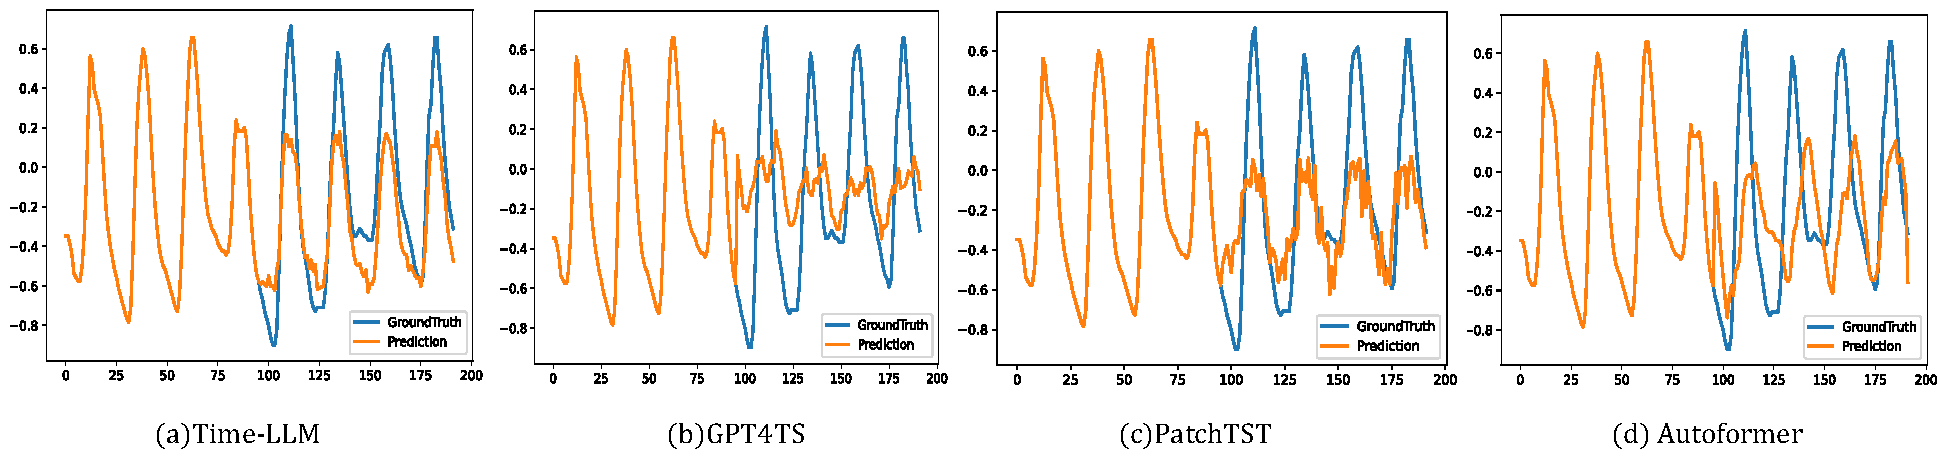
\includegraphics[width=\columnwidth]{figures/visual_zero.pdf}}
	\caption{Zero-shot forecasting cases from ETTh1$\rightarrow$ETTh2 by different models under the input-96-predict-96 settings. \textcolor{blue}{Blue} lines are the ground truths and \textcolor{orange}{orange} lines are the model predictions.}
	\label{fig:visual_etth1_etth2}
\end{center}
\vspace{-20pt}
\end{figure*}